\subsection{Business personas: a four-group lens on RFM}
The statistical selection above chooses $k=2$ for every feature space, which separates high from low activity but gives marketing little to act on. As a complementary \emph{interpretive} view we refit K-means on the same standardized log RFM coordinates with $k=4$ (20 initializations, seed 42). This does not replace the $k=2$ result; it re-slices the same activity gradient into groups that are easier to name and target. Personas are ordered by mean monetary value.

\begin{table}[htbp]\centering\small
\caption{RFM personas ($k=4$). Recency, frequency and monetary value are calibration medians (days $\leq500$); the last three columns use the later period (days 501--711), which was not used for clustering.}\label{tab:personas}
\setlength{\tabcolsep}{4pt}\begin{tabular}{lrrrrrrrr}\toprule
Persona & $n$ & \% & Rec. & Freq. & Mon. (\$) & Later spend (\$) & Active (\%) & Share (\%)\\\midrule
Loyal high-value & 679 & 27.2 & 2 & 134 & 4,223 & 2,256 & 99.7 & 56.6\\
Steady regulars & 924 & 37.0 & 5 & 57 & 1,590 & 932 & 99.7 & 31.8\\
Occasional shoppers & 638 & 25.5 & 18 & 23 & 558 & 416 & 98.1 & 9.8\\
Lapsed / at-risk & 257 & 10.3 & 110 & 7 & 164 & 189 & 83.7 & 1.8\\\bottomrule
\end{tabular}\end{table}
\begin{figure}[htbp]\centering
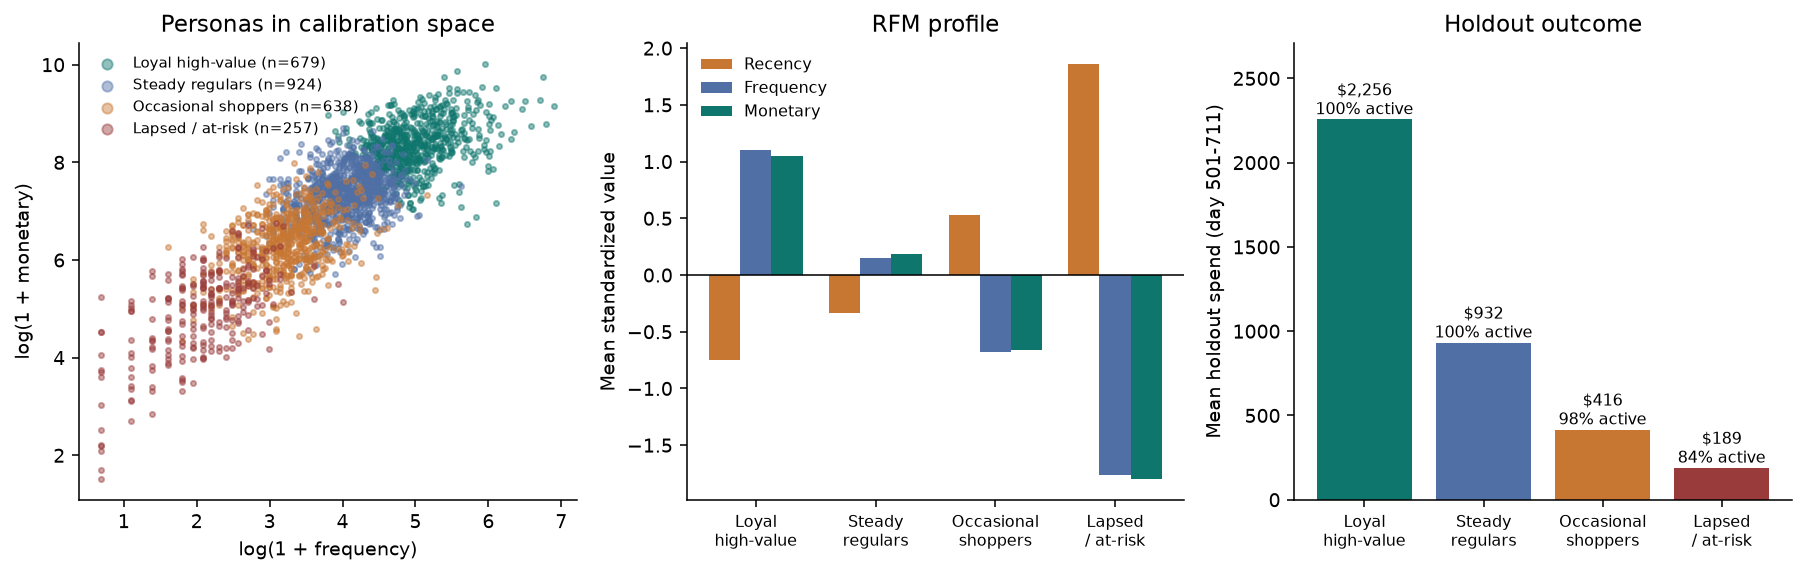
\includegraphics[width=\textwidth]{../figures/13_rfm_personas.png}
\caption{Four RFM personas. Left: households in log frequency--monetary space. Middle: mean standardized R, F and M per persona. Right: mean holdout spend with the share of households that purchased again.}\label{fig:personas}
\end{figure}
\paragraph{Interpretation.} \emph{Loyal high-value} households (679, 27.2\%) shop about 134 times with median spend \$4,223, were last seen a median 2 days before day 500, and account for 56.6\% of later spend. \emph{Steady regulars} (924, 37.0\%) are recent, mid-frequency shoppers contributing 31.8\% of later spend. \emph{Occasional shoppers} (638, 25.5\%) buy roughly 23 times with median recency 18 days. \emph{Lapsed / at-risk} households (257, 10.3\%) have the longest gap since their last purchase (median 110 days), and only 83.7\% purchased in the later period against at least 98.1\% elsewhere.

\paragraph{Implications.} \emph{Loyal high-value}: protect rather than discount; prioritize service quality, early access and loyalty rewards, since losing one costs the most. \emph{Steady regulars}: the main growth pool; use cross-sell and basket-building offers to move them toward the top group. \emph{Occasional shoppers}: raise visit frequency with reminders and targeted coupons for categories they already buy. \emph{Lapsed / at-risk}: low-cost win-back messages with a firm budget cap, as expected payoff is small (mean later spend \$189).

\paragraph{Caveat.} Four groups are weaker than two statistically: over all 2,498 households the silhouette is 0.293 for $k=4$ against 0.451 for $k=2$ (Table~\ref{tab:selected} reports 0.456 for $k=2$ on the fixed 1,500-household evaluation sample). Subsample stability is high on average (mean ARI 0.93) but uneven (range 0.39--1.00 over 20 independent 80\% samples), so individual boundary households can move between neighbouring personas when the gradient is cut at slightly different places. The personas are a descriptive lens for communication and targeting, not evidence of four natural household types, and the labels are our interpretation of the numbers.
